\documentclass{article}
\usepackage[margin=1.2in]{geometry}
\usepackage{parskip}
\usepackage[pdftex]{graphicx}
\usepackage{epsfig}
\usepackage[utf8]{inputenc}
\usepackage[T1]{fontenc}
\usepackage{amsthm}
\usepackage{color}
\usepackage[usenames,dvipsnames]{xcolor}
\usepackage{textcomp}
\usepackage{url}
\definecolor{listinggray}{gray}{0.9}
\definecolor{lbcolor}{rgb}{0.9,0.9,0.9}
\usepackage{listings}
\usepackage{textcomp}
\usepackage{algpseudocode}
\pagestyle{plain}
\topmargin -0.8in
\textheight 9.5in
\oddsidemargin -0.1in
\textwidth 6.8in

\title{\Huge{\textbf{Movie Recommendation System}}}
\author{\normalsize Ankur Garg, Chirag Gupta, Pankaj More, Pranjal Singh\\
\emph{Indian Institute of Technology,Kanpur}}

\date{\today}
\begin{document}
\maketitle
\begin{abstract}
Recommendation System can provide suggestions about movies, videos, newspaper articles to a user. For instance, they may predict whether a user would like a movie or not. These systems collects information from a large number of users and mainly use nearest neighbor techniques to provide recommendations. In this project, we have built a movie-recommendation system using MovieLens Database. We have tried building and using several systems which mainly use a Machine Learning approach called Collaborative filtering. We have tried both the approaches, Item Based and User Based Collaborative filtering and compared the results with the already developed systems.
\end{abstract}

\section{Introduction}
With the explosion of Internet Technologies and arrival of Websites such as IMDB, user demand has taken a new turn where they are facing with problem of too much choice. There is a lot of information available everywhere but user doesn't know which one to go for. Same is the case with movies, where a user has a large number of choices but he doesn't know which one to go for. In many cases, they select an option which is very similar to a person with same preferences and also very consistent to his/her past preferences. This basic phenomenon can be exploited to build a system which can solve this dilemma of large number of choices for a user. A number of such systems have been developed but none can guarantee that a user agrees with the choice they provide.\\ 

Recommendation Systems are special type of systems that combine the knowledge of user's preferences with the knowledge of other similar users to filter the choices and provide most relevant information. Two main approaches of filtering content based approach and collaborative approach. A content based recommendation system uses the user’s past history to recommend new items where as a collaborative approach uses the preferences of other people with similar tastes for recommending items to the user. Recommender systems are a useful alternative to search algorithms since they help users discover items they might not have found by themselves.\\ 

We have tried with several approaches using Item Based and User Based Collaborative Filtering on the \emph{100k Movielens Database}. We can predict a movie for a particular user and also predict what rating he is going to give to the movie. The systems have been developed in Java and Python and currently uses a simple console based interface. Evaluation is important in assessing the effectiveness of recommendation algorithms. So we have used Root Mean Squared Error and Mean Absolute Error metrics to evaluate our results.

\section{Collaborative Filtering}
Collaborative filtering is a method of making automatic predictions (filtering) about the interests of a user by collecting preferences or taste information from many users (collaborating). The underlying assumption of the collaborative filtering approach is that if a person A has the same opinion as a person B on an issue, A is more likely to have B's opinion on a different issue x than to have the opinion on x of a person chosen randomly.
Various Approaches for Collaborative Filtering are as follows:
\subsection{Random Recommendation}
It produces random recommendations and preference estimates. This is likely only useful as a novelty and for benchmarking . It should produce worst result of all the algorithms.

\subsection{User-Based Recommendation}
User-based Collaborative Filtering (UCF) is one of most popular recommendation technique. Given an unknown test rating (of a test item by a test user) to be estimated, user-based collaborative filtering measures similarities between test user and other users

\subsection{Item-Based Recommendation}
Item-based collaborative filtering is a model-based algorithm for making recommendations. In the algorithm, the similarities between different items in the dataset are calculated by using one of a number of similarity measures, and then these similarity values are used to predict ratings for user-item pairs not present in the dataset.

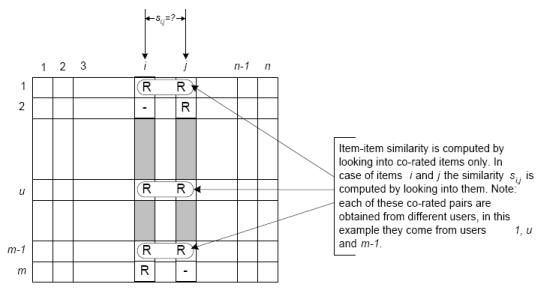
\includegraphics[width=15cm]{image.jpg}

\subsection{Slope–One Recommendation}
It estimates preferences for new items based on average difference in preference value (“diffs”) between a new item and the other items the user prefers. The algorithm consists of a significant preprocessing phase, in which all item-item preference value differences are computed:\\ \\
\textbf{begin}\\
\textbf{for} every item \emph{i}\\
\textbf{for} every other item \emph{j}\\
\textbf{for} every user \emph{u} expressing preference for both \emph{i} and \emph{j}\\
\textbf{add} the difference in \emph{u’s} preference for \emph{i} and \emph{j} to an average\\

And then, the recommendation algorithm becomes:\\ \\
\textbf{for} every item \emph{i} the user \emph{u} expresses no preference for\\
\textbf{for} every item \emph{j} that user \emph{u} expresses a preference for\\
Find the average preference difference between \emph{j} and \emph{i}\\
\textbf{add} this diff to \emph{u’s} preference value for \emph{j}\\
\textbf{add} this to a running average\\
\textbf{return} the top items, ranked by these averages \\

\subsection{Item Average Recommendation}
A simple recommender that always estimates preference for an item to be the average of all known preference values for that item. No information about users is taken into account. This implementation is provided for experimentation; while simple and fast, it may not produce very good recommendations.

\subsection{Item-User Average recommendation}
Like Item Average Recommender, except that estimated preferences are adjusted for the users' average preference value. For example, say user X has not rated item Y. Item Y's average preference value is 3.5. User X's average preference value is 4.2, and the average over all preference values is 4.0. User X prefers items 0.2 higher on average, so, the estimated preference for user X, item Y is 3.5 + 0.2 = 3.7.


\section{Trade- Off Between User-Based Recommendation and Item-Based Recommendation}
The throughput of User-Based Recommendation System decrease as the number of users increases. For Example, it may take a large time predict a value in a large network like internet. But the number of items may be small , thus Item Based Recommendation may work well .Similarly in the case of Item Based Recommendation, it may not be fruitful to calculate the similarity between hundreds of item for example in case of music albums there can be 1000s of song tracks and may be only some users .Thus in this case user based recommendation may work well.


\section{Results}

\subsection{User Based Collaborative Filtering}

\subsubsection{Pearson Correlation Similarity}
\begin{figure}[h!tb]
\centering
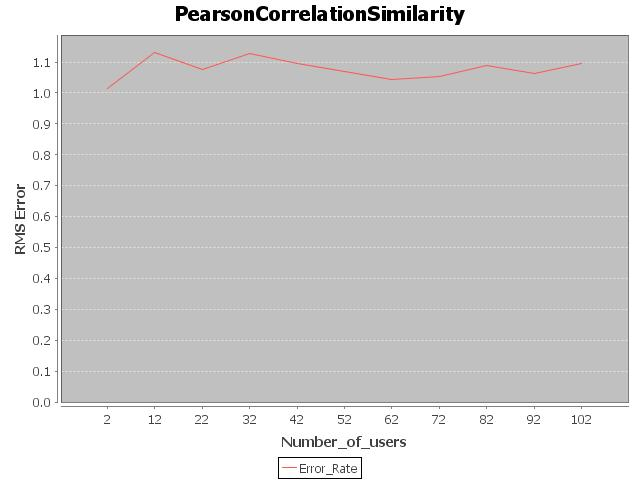
\includegraphics[height=6cm,width=11cm]{1.jpg}
\caption {Plot of Number of users vs. RMS Error for Pearson Correlation Coefficient}
\end{figure}
\newpage
\subsubsection{Euclidean Distance Similarity Measure}
\begin{figure}[h!tb]
\centering
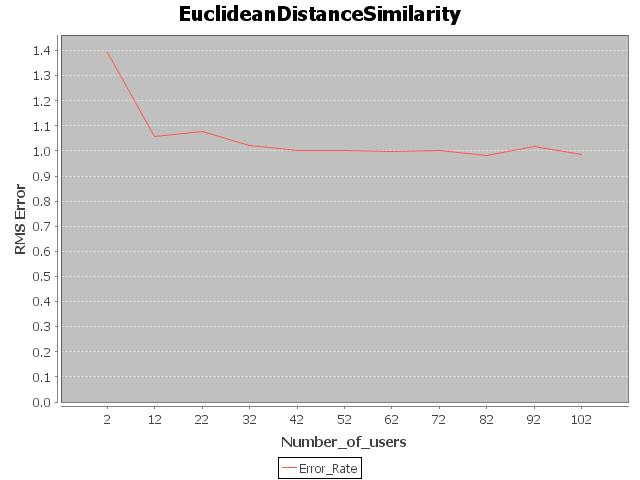
\includegraphics[width=11cm]{2.jpg}
\caption {Plot of Number of users vs. RMS Error for Euclidean Distance Similarity}
\end{figure}

\subsubsection{Cosine Distance Similarity Measure}
\begin{figure}[h!tb]
\centering
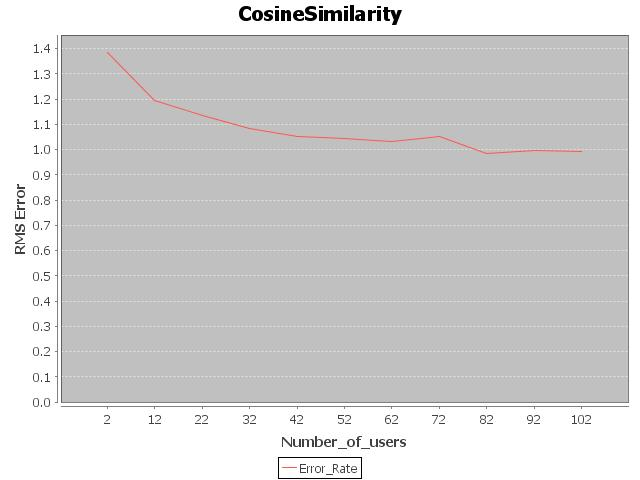
\includegraphics[width=11cm]{3.jpg}
\caption {Plot of Number of users vs. RMS Error for Cosine Similarity}
\end{figure}
\newpage
\subsubsection{k-NN u1base/test to u5base/test}
\begin{figure}[h!tb]
\centering
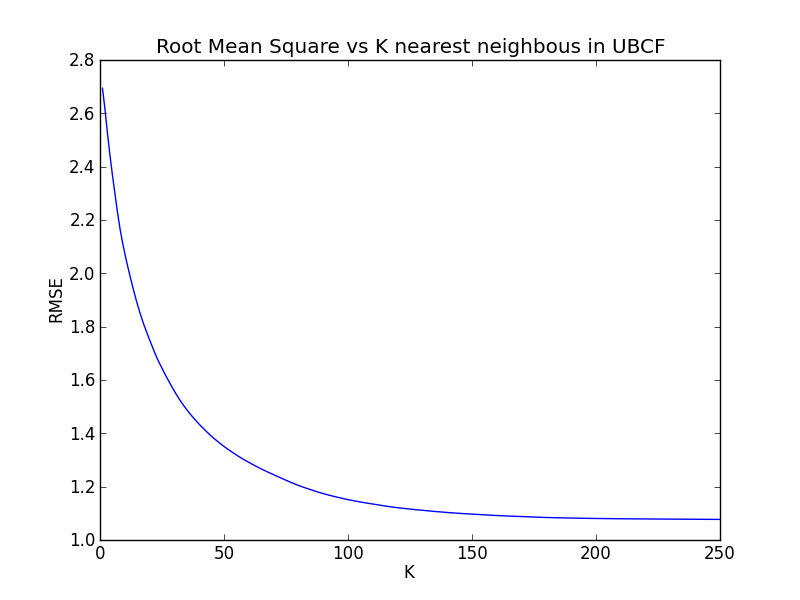
\includegraphics[width=11cm]{6.png}
\caption {u1base/test}
\end{figure}
\begin{figure}[h!tb]
\centering
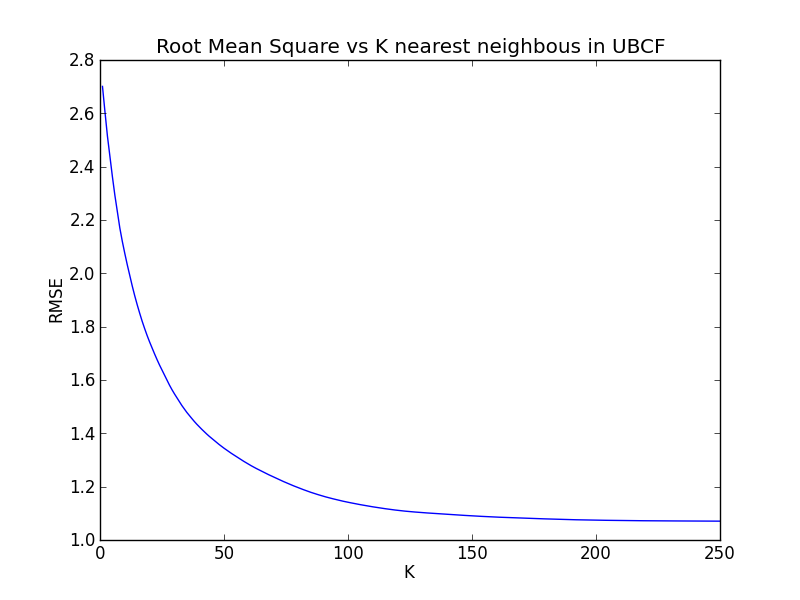
\includegraphics[width=11cm]{7.png}
\caption {u2base/test}
\end{figure}
\newpage
\begin{figure}[h!tb]
\centering
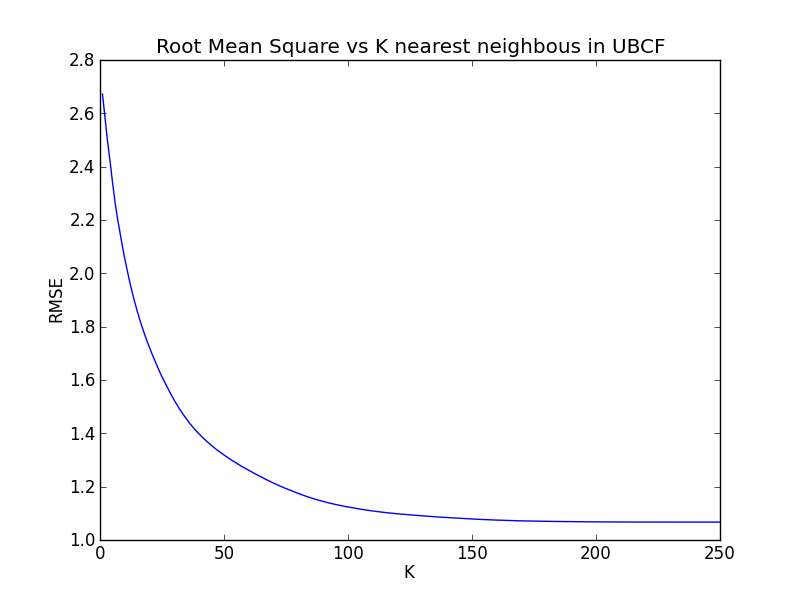
\includegraphics[width=11cm]{8.png}
\caption {u3base/test}
\end{figure}
\begin{figure}[h!tb]
\centering
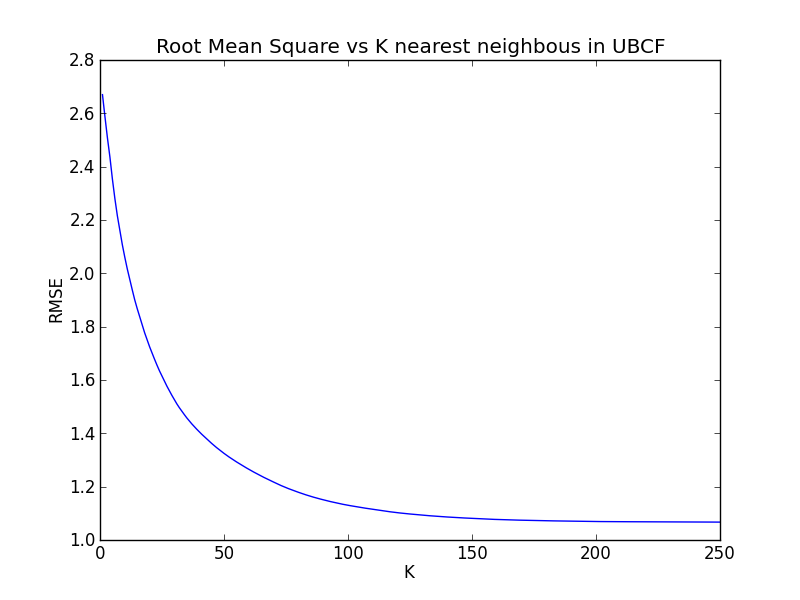
\includegraphics[width=11cm]{9.png}
\caption {u4base/test}
\end{figure}
\begin{figure}[h!tb]
\centering
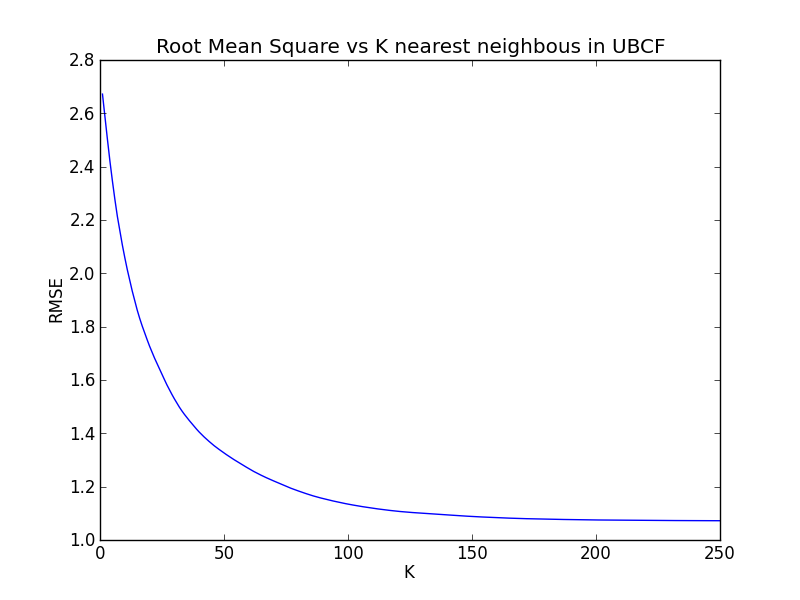
\includegraphics[width=11cm]{10.png}
\caption {u5base/test}
\end{figure}
\newpage
\subsection{Item Based Collaborative Filtering}
\begin{figure}[h!tb]
\centering
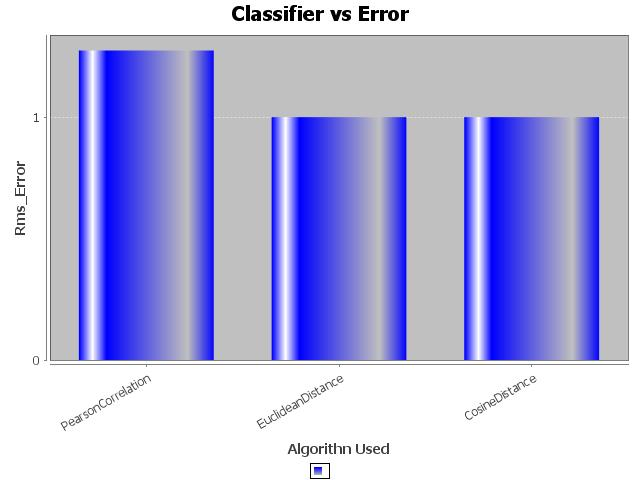
\includegraphics[width=11cm]{4.jpg}\\
\caption {Plot of Result of Item-Based Recommendation based on Different Similarity Techniques}
\end{figure}
\begin{figure}[h!tb]
\centering
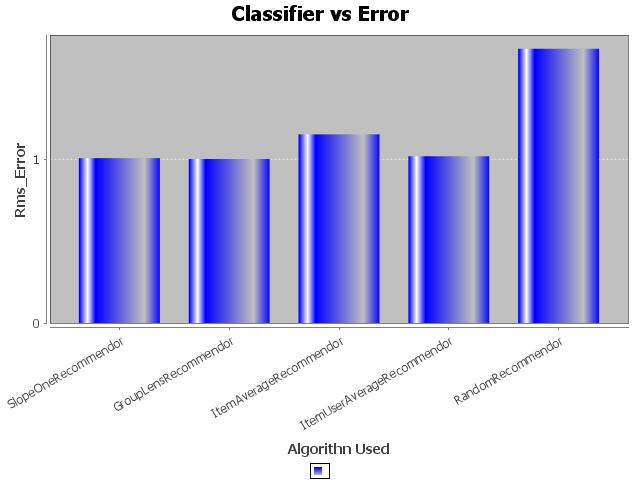
\includegraphics[width=11cm]{5.jpg}
\caption {Plot of Result of Different Recommendation Algorithms based}
\end{figure}

\subsection{Table}

\begin{tabular}{| l | l | l |}
\hline
\textbf{S.No.} & \textbf{Algorithm Used} & \textbf{RMS Error Found} \\ \hline
1 & Random Recommender & 1.706745107579322 \\ \hline
2 & GroupLens Recommender & 0.9604833884849696 \\ \hline
3 & Item Average Recommender & 1.046489529489477 \\ \hline
4 & Item User Average Recommender & 0.992324821381628 \\ \hline
5 & Slope One Recommender & 0.9596826270668479 \\ \hline
6 & Item Based with Pearson Correlation Similarity & 1.2848360576796047 \\ \hline
7 & Item Based with Euclidean Distance Similarity & 1.0270202156297646 \\ \hline
8 & Item Based with Cosine Similarity & 1.0434303652370585 \\ \hline
9 & User Based with Euclidean Distance Similarity(k=50) & 0.9796846711922585 \\ \hline
10 & User Based with Euclidean Distance Similarity(k=100) & 1.0307653814022009 \\ \hline
11 & User Based with Pearson Correlation Similarity (k=50) & 1.077093120362919 \\ \hline
12 & User Based with Pearson Correlation Similarity (k=100) & 1.0768530493114155 \\ \hline
13 & User Based with Cosine Similarity (k=50) & 1.025580177537051 \\ \hline
14 & User Based with Cosine Similarity (k=100) & 1.018564613113902 \\ \hline
\end{tabular}

\section{Conclusion}
\section{References}
\begin{itemize}
\item Java Doc-Mahout Core 0.9 API
\item A Programmer's Guide to Data Mining ($http://guidetodatamining.com/$)
\end{itemize}
\end{document}
